% !TEX TS-program = pdflatex
% !TEX encoding = UTF-8 Unicode

% This is a simple template for a LaTeX document using the "article" class.
% See "book", "report", "letter" for other types of document.

\documentclass[11pt]{article} % use larger type; default would be 10pt

\usepackage[utf8]{inputenc} % set input encoding (not needed with XeLaTeX)

%%% Examples of Article customizations
% These packages are optional, depending whether you want the features they provide.
% See the LaTeX Companion or other references for full information.

%%% PAGE DIMENSIONS
\usepackage{geometry} % to change the page dimensions
\geometry{a4paper} % or letterpaper (US) or a5paper or....
\geometry{margin=1in} % for example, change the margins to 2 inches all round
% \geometry{landscape} % set up the page for landscape
%   read geometry.pdf for detailed page layout information

\usepackage{graphicx} % support the \includegraphics command and options

% \usepackage[parfill]{parskip} % Activate to begin paragraphs with an empty line rather than an indent
\usepackage{amssymb}
\usepackage{amsmath}
%%% PACKAGES
\usepackage{booktabs} % for much better looking tables
\usepackage{array} % for better arrays (eg matrices) in maths
\usepackage{paralist} % very flexible & customisable lists (eg. enumerate/itemize, etc.)
\usepackage{verbatim} % adds environment for commenting out blocks of text & for better verbatim
\usepackage{subfig} % make it possible to include more than one captioned figure/table in a single float
% These packages are all incorporated in the memoir class to one degree or another...

%%% HEADERS & FOOTERS
\usepackage{fancyhdr} % This should be set AFTER setting up the page geometry
\pagestyle{fancy} % options: empty , plain , fancy
\renewcommand{\headrulewidth}{0pt} % customise the layout...
\lhead{}\chead{}\rhead{}
\lfoot{}\cfoot{\thepage}\rfoot{}

%%% SECTION TITLE APPEARANCE
\usepackage{sectsty}
\allsectionsfont{\sffamily\mdseries\upshape} % (See the fntguide.pdf for font help)
% (This matches ConTeXt defaults)

%%% ToC (table of contents) APPEARANCE
\usepackage[nottoc,notlof,notlot]{tocbibind} % Put the bibliography in the ToC
\usepackage[titles,subfigure]{tocloft} % Alter the style of the Table of Contents
\usepackage{bbm}
\usepackage{endnotes}

\renewcommand{\cftsecfont}{\rmfamily\mdseries\upshape}
\renewcommand{\cftsecpagefont}{\rmfamily\mdseries\upshape} % No bold!
\DeclareMathOperator*{\argmax}{arg\,max}
\DeclareMathOperator*{\argmin}{arg\,min}
\usepackage{graphicx}
\graphicspath{ {./pings/} }

\newcount\colveccount
\newcommand*\colvec[1]{
        \global\colveccount#1
        \begin{pmatrix}
        \colvecnext
}
\def\colvecnext#1{
        #1
        \global\advance\colveccount-1
        \ifnum\colveccount>0
                \\
                \expandafter\colvecnext
        \else
                \end{pmatrix}
        \fi
}

\newcommand{\norm}[1]{\left\lVert#1\right\rVert}

\title{Econometrics HW5}
\author{Michael B. Nattinger\footnote{I worked on this assignment with my study group: Alex von Hafften, Andrew Smith, and Ryan Mather. I have also discussed problem(s) with Emily Case, Sarah Bass, Katherine Kwok, and Danny Edgel.}}

\begin{document}
\maketitle

\section{Question 1}
\subsection{Part i}
It is pretty simple to show that $U_t,W_t,V_t$ are mean $0$:
\begin{align*}
E[U_t] &= E[\epsilon_t \epsilon_{t-1}]\\
&= E[\epsilon_{t}]E[\epsilon_{t-1}]\\
&= 0.
\end{align*}
\begin{align*}
E[W_t] &= E[\epsilon_t \epsilon_{0}]\\
&= E[\epsilon_{t}]E[\epsilon_{0}]\\
&= 0.
\end{align*}
\begin{align*}
E[V_t] &= E[\epsilon_t^{2} \epsilon_{t-1}]\\
&= E[\epsilon_{t}^2]E[\epsilon_{t-1}]\\
&= 0.
\end{align*}
We now will find autocovariance functions $\gamma,\psi,\eta$ for $U_t,W_t,V_t$ respectively.
\begin{align*}
\gamma(k) &= Cov(U_t,U_{t-k}) = Cov(\epsilon_t \epsilon_{t-1},\epsilon_{t-k} \epsilon_{t-k-1})  = \begin{cases} 0, k>1\\
Cov(\epsilon_{t} \epsilon_{t-1}, \epsilon_{t-1} \epsilon_{t-2}) = E[\epsilon_t \epsilon_{t-2} \epsilon_{t-1}^2] = 0, k=1\\
Cov(\epsilon_{t} \epsilon_{t-1}, \epsilon_{t} \epsilon_{t-1}) = E[\epsilon_{t}^2 \epsilon_{t-1}^2] = \sigma^4 , k = 0
\end{cases} \\
\psi(k) &=Cov(W_t,W_{t-k}) = Cov(\epsilon_t \epsilon_{0},\epsilon_{t-k} \epsilon_{0}) = \begin{cases} E[\epsilon_t \epsilon_{0}^2\epsilon_{t-k}] = 0, k>0\\
E[\epsilon_{t}^2 \epsilon_{0}^2] = \sigma^4 , k = 0
\end{cases} \\
\eta(k) &= Cov(V_t,V_{t-k}) = Cov(\epsilon_t^2 \epsilon_{t-1},\epsilon_{t-k}^2 \epsilon_{t-k-1})  = \begin{cases} 0, k>1\\
E[\epsilon_t^2 \epsilon_{t-1}^3 \epsilon_{t-2}] = 0, k=1\\
 E[\epsilon_t^4 \epsilon_{t-1}^2 ]  = \sigma^2E[\epsilon_t^4] , k = 0
\end{cases} 
\end{align*}
Therefore, $U_t,W_t,V_t$ all have autocovariance functions and are covariance stationary.

\subsection{Part ii}
\begin{align*}
Var(\bar{U}) &= Var\left(\frac{1}{T}\sum_{t=1}^{T}U_t\right) \\
&= \frac{1}{T}Var(U_t)\\
&= \frac{\sigma^4}{T} \\
&\rightarrow  0
\end{align*}
The same is true for $Var(\bar{W}),Var(\bar{V})$ by the same logic. Therefore, $\bar{U},\bar{V},\bar{W}$ all converge in probability to their means (0).
\subsection{Part iii}
\begin{align*}
Var(\hat{\gamma}_{U}(0)) &= Var(\frac{1}{T}\sum_{t=1}^{T}U_t^2) \\
&= \frac{1}{T}Var(U_t^2)\\
&= \frac{1}{T}Var(\epsilon_t^2\epsilon_{t-1}^2)\\
&= \frac{E[\epsilon_t^4\epsilon_{t-1}^4] - E[\epsilon_t^2\epsilon_{t-1}^2]^2}{T}\\
&=  \frac{E[\epsilon_t^4]E[\epsilon_{t-1}^4] - E[\epsilon_t^2]^2E[\epsilon_{t-1}^2]^2}{T} \\
&=  \frac{E[\epsilon_t^4]E[\epsilon_{t-1}^4] - \sigma^8}{T}\\
&\rightarrow 0. 
\end{align*}
\begin{align*}
Var(\hat{\gamma}_{W}(0)) &= Var(\frac{1}{T}\sum_{t=1}^{T}W_t^2) \\
&= \frac{1}{T}Var(W_t^2)\\
&= \frac{1}{T}Var(\epsilon_t^2\epsilon_{0}^2)\\
&= \frac{E[\epsilon_t^4\epsilon_{0}^4] - E[\epsilon_t^2\epsilon_{0}^2]^2}{T}\\
&=  \frac{E[\epsilon_t^4]E[\epsilon_{0}^4] - E[\epsilon_t^2]^2E[\epsilon_{0}^2]^2}{T} \\
&=  \frac{E[\epsilon_t^4]E[\epsilon_{0}^4] - \sigma^8}{T}\\
&\rightarrow 0. 
\end{align*}
\begin{align*}
Var(\hat{\gamma}_{V}(0)) &= Var(\frac{1}{T}\sum_{t=1}^{T}V_t^2) \\
&= \frac{1}{T}Var(V_t^2)\\
&= \frac{1}{T}Var(\epsilon_t^4\epsilon_{t-1}^2)\\
&= \frac{E[\epsilon_t^8\epsilon_{t-1}^4] - E[\epsilon_t^4\epsilon_{t-1}^2]^2}{T}\\
&=  \frac{E[\epsilon_t^8]E[\epsilon_{t-1}^4] - E[\epsilon_t^4]^2E[\epsilon_{t-1}^2]^2}{T} \\
&\rightarrow 0. 
\end{align*}
So, these are converging to point masses. However, note that:
\begin{align*}
\hat{\gamma}_{W}(0) &= \frac{1}{T}\sum_{t=1}^{T}W_t^2\\
&=\epsilon_{0}^2  \frac{1}{T}\sum_{t=1}^{T}\epsilon_t^2\\
&\rightarrow_p \epsilon_{0}^2 \sigma^2.
\end{align*}
This is clearly not its expectation:
\begin{align*}
E[\hat{\gamma}_{W}(0)] &= E\left[\frac{1}{T}\sum_{t=1}^{T}W_t^2\right]\\
&=  \frac{1}{T}\sum_{t=1}^{T}E\left[\epsilon_t^2\epsilon_{0}^2\right]\\
&= E[\epsilon_t^2] E[\epsilon_0^2]\\
&= \sigma^4.
\end{align*}
The other estimators clearly do converge to their expectations.
%\begin{align*}
%\hat{\gamma}_{V}(0) &= \frac{1}{T}\sum_{t=1}^{T}V_t^2\\
%&=frac{1}{T}\sum_{t=1}^{T}\epsilon_t^2 \epsilon_{t-1}^2\\
%&\rightarrow_p 
%\end{align*}

\subsection{Part iv}
From the above, we know that $\bar{W}$ does not converge to its expectation, so we cannot use our Martingale CLT on $\sqrt{T}\bar{W}$. It is, in fact, not asymptotically normal:
\begin{align*}
\sqrt{T}\bar{W} &= \epsilon_0 \frac{1}{\sqrt{T}}\sum_{t=1}^T \epsilon_t
\end{align*}

$\frac{1}{\sqrt{T}}\sum_{t=1}^T \epsilon_t$ is normal, but $\epsilon_0$ is random and in general the product of a normal with another arbitrary random variable is not normal. Therefore, $\sqrt{T}\bar{W}$ is not normal.

We know that $U_t$ is strictly stationary with finite second moment and convergence in probability of the second sample moment. Moreover,

\begin{align*}
E[U_t|U_{t-1},\dots,U_1] &= E[E[\epsilon_t\epsilon_{t-1}|\epsilon_{t-1},\dots,\epsilon_0]|U_{t-1},\dots,U_1] \\
&= E[\epsilon_{t-1} (0) |U_{t-1},\dots,U_1]\\
&= 0.
\end{align*}

Therefore, we can use the martingale CLT and $\sqrt{T}\bar{U}\rightarrow_d N(0,\sigma^4)$

We know that $V_t$ is strictly stationary with finite second moment and convergence in probability of the second sample moment. Note that the conditioning trick that we used before will not work with $V_t$. Instead, we denote $\tilde{V}_t = V_{T-t+1}$ and work backwards:

\begin{align*}
E[\tilde{V}_t|\tilde{V}_{t-1},\dots,\tilde{V}_1] &=E[E[\epsilon_{T-t+1}^2\epsilon_{T-t}|\epsilon_T,\dots,\epsilon_{T-t+1}]|\tilde{V}_{t-1},\dots,\tilde{V}_1]\\
&=E[\epsilon_{T-t+1}^2(0)|\tilde{V}_{t-1},\dots,\tilde{V}_1]\\
&= 0.
\end{align*}

Therefore, we can use the martingale CLT and prove that $\sqrt{T}V$ is asymptotically normal.

\section{Question 2}
\subsection{Part i}
The time series is easily simulated in Matlab. Code screenshots follow at the end of the problem set. Results from the first simulation are below:

\begin{centering}
\begin{tabular}{llllllllll}
& $\hat{\alpha}_0$ & $\hat{\alpha}_0$ LB & $\hat{\alpha}_0$ UB & $\hat{\delta}_0$ & $\hat{\delta}_0$ LB & $\hat{\delta}_0$ UB & $\hat{\rho}_1$ & $\hat{\rho}_1$ LB & $\hat{\rho}_1$ UB \\ 
\hline 
$(T=50,\rho_1=0.7)$ & 2.04 & 1.33 & 2.75 & 0.984 & 0.646 & 1.32 & 0.507 & 0.317 & 0.696 \\ 
$(T=50,\rho_1=0.9)$ & 1.68 & 0.762 & 2.6 & 0.835 & 0.598 & 1.07 & 0.883 & 0.787 & 0.98 \\ 
$(T=50,\rho_1=0.95)$ & 1.34 & 0.813 & 1.86 & 1.41 & 1.14 & 1.68 & 0.911 & 0.825 & 0.998 \\ 
$(T=150,\rho_1=0.7)$ & 0.956 & 0.605 & 1.31 & 1.08 & 0.943 & 1.23 & 0.67 & 0.591 & 0.749 \\ 
$(T=150,\rho_1=0.9)$ & 1.32 & 0.803 & 1.83 & 0.885 & 0.723 & 1.05 & 0.896 & 0.855 & 0.937 \\ 
$(T=150,\rho_1=0.95)$ & 0.918 & 0.462 & 1.38 & 0.853 & 0.696 & 1.01 & 0.95 & 0.925 & 0.974 \\ 
$(T=250,\rho_1=0.7)$ & 1.36 & 1.04 & 1.67 & 1.02 & 0.913 & 1.13 & 0.616 & 0.552 & 0.68 \\ 
$(T=250,\rho_1=0.9)$ & 0.873 & 0.608 & 1.14 & 0.96 & 0.837 & 1.08 & 0.909 & 0.879 & 0.938 \\ 
$(T=250,\rho_1=0.95)$ & 1.19 & 0.888 & 1.49 & 1.02 & 0.905 & 1.13 & 0.921 & 0.891 & 0.951 \\ 
\hline 
\end{tabular}
\end{centering}
\subsection{Part ii}
Results from repeating the simulation 10000 times are below:

\begin{centering}
\begin{tabular}{lllllll}
& $\hat{\alpha}_0$ Mean & $\hat{\alpha}_0$ Coverage & $\hat{\delta}_0$ Mean & $\hat{\delta}_0$ Coverage & $\hat{\rho}_1$ Mean & $\hat{\rho}_1$ Coverage \\ 
\hline 
$(T=50,\rho_1=0.7)$ & 1.09 & 0.901 & 1 & 0.916 & 0.659 & 0.89 \\ 
$(T=50,\rho_1=0.9)$ & 1.16 & 0.866 & 0.995 & 0.916 & 0.853 & 0.844 \\ 
$(T=50,\rho_1=0.95)$ & 1.13 & 0.843 & 0.991 & 0.915 & 0.897 & 0.802 \\ 
$(T=150,\rho_1=0.7)$ & 1.04 & 0.939 & 1 & 0.939 & 0.687 & 0.93 \\ 
$(T=150,\rho_1=0.9)$ & 1.09 & 0.921 & 1 & 0.938 & 0.887 & 0.913 \\ 
$(T=150,\rho_1=0.95)$ & 1.11 & 0.908 & 1 & 0.943 & 0.937 & 0.892 \\ 
$(T=250,\rho_1=0.7)$ & 1.03 & 0.939 & 1 & 0.945 & 0.692 & 0.937 \\ 
$(T=250,\rho_1=0.9)$ & 1.06 & 0.929 & 1 & 0.944 & 0.892 & 0.928 \\ 
$(T=250,\rho_1=0.95)$ & 1.08 & 0.922 & 1 & 0.943 & 0.942 & 0.914 \\ 
\hline 
\end{tabular}
\end{centering}
\subsection{Part iii}
It is clear from the simulation results that the estimated OLS coefficients are, on average, closer to the true value and are more often covered by the confidence interval as $T$ increases. As the degree of persistence of $Y_t$ is closer to $1$, the bias of OLS tends to increase as measured by the coverage percentages falling. It seems likely, in my opinion, that the underperformance of the coverage ratios is caused by bias in the point estimates, as opposed to misidentification of the variance estimates.

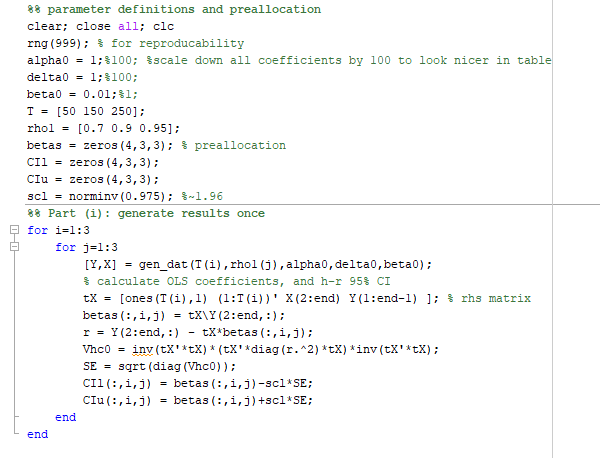
\includegraphics{hw5p1}

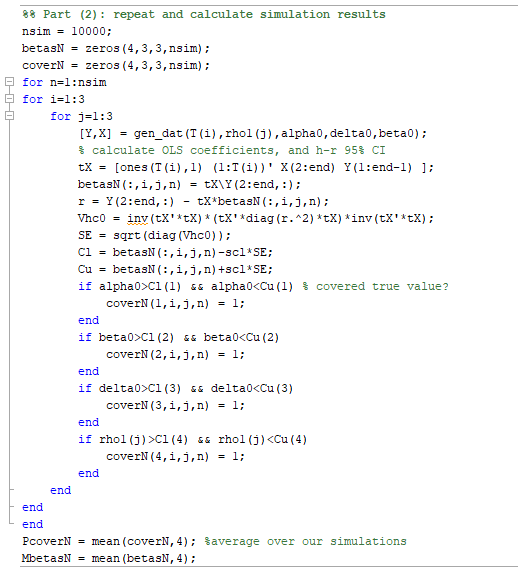
\includegraphics{hw5p2}

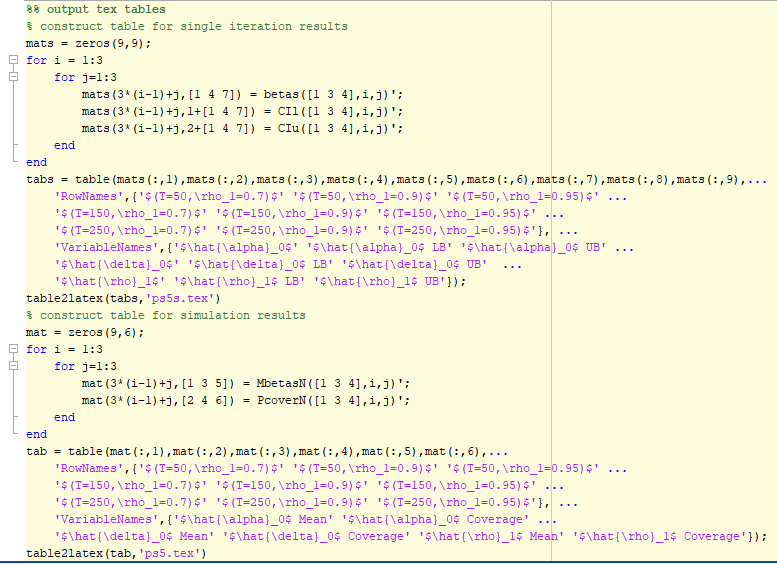
\includegraphics{hw5p3}

Data was generated using the following function:

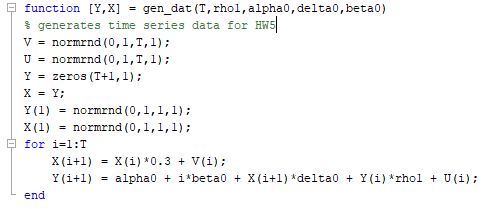
\includegraphics{hw5p4}

\end{document}
